\documentclass[tikz,border=10pt]{standalone}

\usepackage{tikz}
\usetikzlibrary{positioning}
\usetikzlibrary{shapes,arrows,backgrounds,fit,shapes.geometric,calc}
\usetikzlibrary{pgfplots.groupplots}
\usepackage{pgfplots}
\usepackage{pgfplotstable}
\usepackage{listings}
\usepackage{lstautogobble}
\usepackage{color}
\usepackage{amsmath}

\lstset{
    language=[ANSI]C++,
    basicstyle=\small\ttfamily,
    identifierstyle=\color{black}\small\ttfamily,
    keywordstyle=\color{red}\small\ttfamily,
    commentstyle=\color{green!30!black}\bf\small\ttfamily,
    breaklines=true
}

\tikzset{
    %Define standard arrow tip
    >=stealth',
    % Define arrow style
    pil/.style={
           ->,
       thick,}
           %shorten <=2pt,
           %shorten >=2pt,}
}

\newcommand{\execwidth}{2cm}

\begin{document}
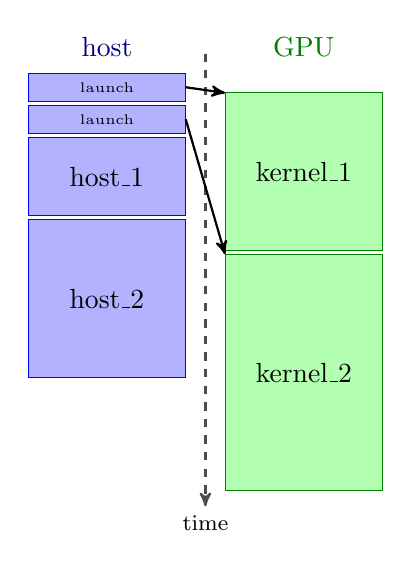
\begin{tikzpicture}[x=0cm, y=0cm, node distance=0 cm,outer sep = 0pt]
\tikzstyle{cpukernel}=[
                  draw=blue,
                  rectangle,
                  minimum width=\execwidth,
                  fill=blue!30,
                  anchor=north west]

\tikzstyle{gpukernel}=[
                  draw=green!50!black,
                  rectangle,
                  minimum width=\execwidth,
                  fill=green!30,
                  anchor=north west]

\node[rectangle] (CPUlabel)  at(1cm,0.1cm) [anchor=south] {\color{blue!50!black}{host}};
\node[rectangle] (GPUlabel)  at(3.5cm,0.1cm) [anchor=south] {\color{green!50!black}{GPU}};

\node[cpukernel] (launch1) at(0,0) [minimum height=0.25cm] {\tiny launch};
\node[cpukernel] (launch2) [below = 0.05cm of launch1, minimum height=0.25cm] {\tiny launch};

\node[cpukernel] (host1)   [below = 0.05cm of launch2, minimum height=1cm] {host\_1};
\node[cpukernel] (host2)   [below = 0.05cm of host1,   minimum height=2cm] {host\_2};

\node[gpukernel] (kernel1) at(2.5cm,-0.25cm) [minimum height=2cm] {kernel\_1};
\node[gpukernel] (kernel2)  [below = 0.05cm of kernel1, minimum height=3cm] {kernel\_2};

\path[pil,->,black!70,dashed] (2.25cm,0.25cm)  edge (2.25cm, -5.5cm);
\node[rectangle] (timelabel)  at(2.25cm,-5.5cm) [anchor=north] {\footnotesize time};

\path[pil,->,black] (launch1.east)  edge (kernel1.north west);
\path[pil,->,black] (launch2.east)  edge (kernel2.north west);

\end{tikzpicture}

\end{document}

